\documentclass[conference]{IEEEtran}
\usepackage[utf8]{inputenc}
\usepackage[T1]{fontenc}
\usepackage[english, portuguese]{babel}
\usepackage{graphicx}   % para incluir figuras
\usepackage{booktabs}   % para tabelas com \toprule, \midrule, \bottomrule
\graphicspath{{./}{resultados/}}  % procura figuras na raiz e em resultados/

\begin{document}
    
    \title{Classificação de Gênero Musical com MLP e CNN: Uma Comparação no Dataset GTZAN}
    
    \author{
        \IEEEauthorblockN{
            Breno Back dos Santos Miranda da Silva (Matrícula: 190063980) \\
            Leonardo Pereira Côrtes (Matrícula: 200030582) \\
            Mariana Soares Oliveira (Matrícula: 231013663) \\
            Matheus de Souza Fernandes (Matrícula: 231025243)
        }
        \vspace{0.5em}
        \IEEEauthorblockA{\textit{Universidade de Brasília}}
    }
    
    \maketitle
    
    % -------------------------------------------------------
    % ABSTRACT (English)
    % -------------------------------------------------------
    \renewcommand{\abstractname}{Abstract}
    \begin{abstract}
        % [TODOS] ~150 palavras em inglês.
        % Cobrir: objetivo, dataset, métodos (MLP e CNN), principais resultados, conclusão.
        This paper presents a comparison between...
    \end{abstract}
    
    \renewcommand{\IEEEkeywordsname}{Keywords}
    \begin{IEEEkeywords}
        Music genre classification, GTZAN, MLP, CNN, MFCC, spectrogram.
    \end{IEEEkeywords}
    
    \vspace{1em}
    
    % -------------------------------------------------------
    % RESUMO (Português)
    % -------------------------------------------------------
    \renewcommand{\abstractname}{Resumo}
    \begin{abstract}
        % [TODOS] Tradução do abstract acima.
        Este artigo apresenta uma comparação entre...
    \end{abstract}
    
    \renewcommand{\IEEEkeywordsname}{Palavras-chave}
    \begin{IEEEkeywords}
        Classificação de gênero musical, GTZAN, MLP, CNN, MFCC, espectrograma.
    \end{IEEEkeywords}
    
    % -------------------------------------------------------
    % I. INTRODUÇÃO
    % -------------------------------------------------------
    \section{Introdução}
    
    A classificação automática de gênero musical é uma tarefa cada vez mais importante devido ao crescimento das plataformas de \textit{streaming} e à necessidade de organizar grandes catálogos de áudio. No entanto, classificar músicas por gênero é um desafio prático, pois os estilos musicais são conceitos bastante subjetivos. Músicas de um mesmo estilo podem soar de formas muito diferentes (devido à alta variabilidade intra-gênero), e gêneros distintos podem compartilhar características acústicas parecidas, dificultando a separação das categorias.
    
    O objetivo deste artigo é comparar o desempenho de duas redes neurais diferentes na classificação de gêneros musicais, utilizando o dataset GTZAN~\cite{tzanetakis2002}. A primeira abordagem utiliza dados tabulares com as características acústicas do áudio para treinar um \textit{Multilayer Perceptron} (MLP). Já a segunda abordagem utiliza os espectrogramas das músicas, tratando o problema como uma tarefa de visão computacional para treinar uma Rede Neural Convolucional (CNN). Com isso, o trabalho busca avaliar qual formato de entrada e arquitetura apresenta os melhores resultados.
    
    O artigo está organizado da seguinte forma: a Seção II apresenta trabalhos relacionados na área; a Seção III descreve o dataset e os métodos de pré-processamento aplicados; a Seção IV detalha a construção dos modelos MLP e CNN; a Seção V mostra os resultados alcançados; a Seção VI discute o desempenho das abordagens e, por fim, a Seção VII finaliza o artigo com a conclusão.
    
    % -------------------------------------------------------
    % II. TRABALHOS RELACIONADOS
    % -------------------------------------------------------
    \section{Trabalhos Relacionados}
    Diversos estudos exploraram a classificação de gênero musical utilizando diferentes representações de entrada. Para a extração de características acústicas tabulares, os coeficientes MFCC (\textit{Mel-Frequency Cepstral Coefficients}) são amplamente consolidados na literatura de processamento de áudio. Logan~\cite{logan2000} demonstrou a eficácia dos MFCCs para a modelagem musical, destacando sua capacidade de capturar a envoltória espectral do som de forma análoga à percepção auditiva humana, tornando-se o padrão de entrada para redes como o \textit{Multilayer Perceptron} (MLP) em tarefas de áudio.
    
    Na abordagem visual, Costa et al.~\cite{costa2017} avaliaram redes neurais convolucionais aplicadas a espectrogramas para classificação musical, demonstrando que tratar o áudio como uma imagem e delegar a extração de características à própria rede pode superar descritores acústicos projetados manualmente. O presente trabalho segue essa linha na abordagem CNN e a contrasta diretamente com um modelo tabular (MLP) treinado sobre descritores MFCC.
    
    % -------------------------------------------------------
    % III. DATASET E PRÉ-PROCESSAMENTO
    % -------------------------------------------------------
    \section{Dataset e Pré-processamento}
    
    \subsection{GTZAN Dataset}
    
    Os experimentos deste projeto utilizaram o dataset GTZAN~\cite{tzanetakis2002}, um dos bancos de dados mais conhecidos para pesquisas em processamento de áudio. O conjunto contém 1000 clipes, distribuídos igualmente em 10 gêneros musicais (100 amostras por categoria). Cada arquivo de áudio possui 30 segundos de duração.
    
    \subsection{Divisão dos Dados}
    
    Ao utilizar o GTZAN, é essencial tratar o alto risco de \textit{data leakage} (vazamento de dados). Isso ocorre porque o dataset possui diversos clipes que foram recortados de trechos diferentes de uma mesma música. Se a divisão dos dados em subconjuntos fosse totalmente aleatória, o modelo poderia ver uma parte da música no treinamento e outra parte da mesma música no teste. Isso faria a acurácia saltar artificialmente para mais de 90\%, pois a rede estaria memorizando as músicas em vez de aprender os padrões gerais de cada gênero.
    
    Para evitar esse problema, foi realizado um \textit{split} estratificado mantendo uma semente aleatória fixa (\texttt{random\_state=42}). Os dados foram divididos seguindo a proporção de 70\% para treinamento, 15\% para validação e 15\% para teste.
    
    \subsection{Pré-processamento Tabular}
    
    Para alimentar a rede MLP, foram utilizadas \textit{features} previamente extraídas, com foco nos coeficientes MFCCs (\textit{Mel-Frequency Cepstral Coefficients}). Colunas que não agregam informação para a classificação computacional, como o nome do arquivo e a duração da faixa, foram removidas.
    
    A normalização dos valores foi feita com a função \texttt{StandardScaler}. Para garantir que dados do futuro não influenciassem o aprendizado, o escalonador foi ajustado (\texttt{fit}) exclusivamente com o conjunto de treino. Só então a transformação foi aplicada para colocar os conjuntos de validação e teste na mesma escala.
    
    \subsection{Pré-processamento de Imagens}
    
    Na abordagem com a CNN, os dados de entrada foram os espectrogramas das músicas originais. Para adequar as imagens ao modelo e otimizar o processamento, elas foram convertidas para escala de cinza e redimensionadas para a resolução de 128 \times 128 pixels.
    
    Os valores dos pixels foram normalizados, sendo divididos por 255.0 para que ficassem no intervalo entre 0 e 1. Por fim, para que a comparação entre os dois modelos fosse cientificamente justa, a separação das imagens em treino, validação e teste utilizou os exatos mesmos índices gerados no \textit{split} dos dados tabulares.
    
    
    % -------------------------------------------------------
    % IV. METODOLOGIA
    % -------------------------------------------------------
    \section{Metodologia}
    
    \subsection{Modelo Tabular - MLP}
    A abordagem tabular foi desenvolvida utilizando a biblioteca \texttt{scikit-learn}. A arquitetura do \textit{Multilayer Perceptron} (MLP) baseou-se diretamente nas \textit{features} MFCCs extraídas. Para encontrar a arquitetura ideal e mitigar os efeitos de \textit{overfitting}, foi implementada uma busca de hiperparâmetros utilizando a técnica \texttt{RandomizedSearchCV} com validação cruzada estratificada (cv=5) e 20 iterações. O espaço de busca abrangeu variações na topologia da rede (de uma a três camadas ocultas), funções de ativação (ReLU e Tanh), taxa de aprendizado inicial e o fator de regularização L2 (\textit{alpha}).
    
    A configuração de melhor desempenho consistiu em uma arquitetura enxuta, possuindo uma única camada oculta com 128 neurônios, função de ativação ReLU, taxa de aprendizado inicial de 0,01 e um termo de regularização \textit{alpha} de 0,0001, operando sob o otimizador Adam. Além da simplicidade arquitetural, a técnica de \textit{Early Stopping} foi fundamental: o treinamento foi configurado para ser interrompido caso a perda (\textit{loss}) no conjunto de validação não apresentasse melhora por 20 épocas consecutivas. Essa estratégia demonstrou-se altamente eficaz para interromper o aprendizado antes que a rede passasse a memorizar os dados de treino, favorecendo a generalização.
    
    \subsection{Modelo Visual - CNN}
    A rede convolucional foi implementada em Keras e recebe como entrada os espectrogramas em escala de cinza de dimensão 128 \times 128 \times 1. A arquitetura é composta por três blocos convolucionais seguidos de uma cabeça de classificação densa.

    Cada bloco convolucional contém uma camada \texttt{Conv2D} com filtros 3 \times 3 e ativação ReLU (com \textit{padding} do tipo \textit{same}, que preserva a dimensão espacial), seguida de \texttt{MaxPooling2D} 2 \times 2 e \texttt{Dropout} de 0,25. O número de filtros cresce a cada bloco (32, 64 e 128), permitindo que a rede aprenda uma hierarquia de padrões: das texturas locais do espectrograma, nos primeiros blocos, a padrões mais abstratos nos blocos finais. O \textit{pooling} reduz progressivamente a resolução (de 128 para 16) e agrega invariância a pequenos deslocamentos, enquanto o \textit{dropout} atua como regularização, importante dado o número reduzido de amostras de treino.

    Após os blocos convolucionais, os mapas de características são achatados (\texttt{Flatten}) e processados por uma camada \texttt{Dense} de 256 neurônios com ativação ReLU, um \texttt{Dropout} mais agressivo de 0,5 e, por fim, uma camada \texttt{Dense} de 10 neurônios com ativação \textit{softmax}, que produz a distribuição de probabilidade sobre os gêneros.

    O treinamento utilizou o otimizador Adam (\textit{learning rate} inicial de $10^{-3}$) e a função de perda \textit{sparse categorical crossentropy}, com \textit{batches} de 32 amostras por até 50 épocas. Dois \textit{callbacks} controlaram o processo: o \textit{EarlyStopping} (monitorando a acurácia de validação, com paciência de 10 épocas e restauração dos melhores pesos), para conter o \textit{overfitting}, e o \textit{ReduceLROnPlateau} (reduzindo o \textit{learning rate} pela metade após 5 épocas sem melhora na perda de validação), permitindo um ajuste mais fino na fase final do treino.

    \textbf{Sobre a normalização em lote.} A arquitetura originalmente proposta incluía uma camada de \textit{Batch Normalization}~\cite{ioffe2015} após cada convolução. Na prática, entretanto, essa configuração fez o treinamento estagnar em acurácia equivalente ao acaso ($\approx 10\%$ para dez classes). O comportamento é consistente com uma limitação conhecida da técnica em cenários de poucos dados: as estatísticas móveis de média e variância, usadas na inferência, não convergem com o número reduzido de \textit{batches} por época, de modo que a normalização aplicada na validação diverge da aplicada no treino. A remoção das camadas de \textit{Batch Normalization}, mantendo o restante da arquitetura, foi suficiente para estabilizar o treinamento e alcançar os resultados reportados.
    
    % -------------------------------------------------------
    % V. RESULTADOS
    % -------------------------------------------------------
    \section{Resultados}
    
    A Tabela~\ref{tab:resultados} apresenta a acurácia global dos dois modelos desenvolvidos. 
    
    Em relação à abordagem tabular, o modelo MLP apresentou um treinamento estável e eficiente. A Figura~\ref{fig:mlp_curves} ilustra a queda acentuada da função de custo (\textit{loss}) de treinamento e a ascensão da acurácia de validação, que atingiu seu ápice próximo à 20ª época (cerca de 70\%). O mecanismo de \textit{Early Stopping} interrompeu o treinamento em torno da 32ª época, garantindo que o modelo retivesse sua capacidade de generalização máxima antes de apresentar sobreajuste severo. A análise da Figura~\ref{fig:mlp_cm} reforça a precisão da rede: gêneros com assinaturas acústicas peculiares, como \textit{classical} e \textit{jazz}, foram amplamente reconhecidos, chegando a 100\% de acertos no caso da música clássica. As maiores sobreposições ocorreram entre \textit{hiphop} e \textit{reggae} (4 falsos preditivos), e \textit{rock} e \textit{disco} (3 falsos preditivos), evidenciando a limitação dos MFCCs puros em discernir certos padrões rítmicos percussivos semelhantes.

    A CNN atingiu 0,64 de acurácia na validação e 0,51 no teste. A Figura~\ref{fig:cnn_curves} apresenta as curvas de treinamento, nas quais se observam a convergência estável do modelo e um leve \textit{overfitting} a partir da vigésima época, comportamento esperado dado o tamanho reduzido do conjunto de treino. A Figura~\ref{fig:cnn_cm} mostra a matriz de confusão na validação: o gênero \textit{metal} foi o mais bem classificado (F1 de 0,93), seguido de \textit{classical} e \textit{hiphop} (ambos com F1 de 0,80), enquanto \textit{rock} e \textit{country} concentraram os maiores erros (F1 de 0,32 e 0,50, respectivamente), refletindo a maior sobreposição de suas características com as dos demais gêneros.
    
    \begin{table}[h]
        \centering
        \caption{Acurácia nos conjuntos de Validação e Teste}
        \label{tab:resultados}
        \begin{tabular}{lcc}
            \toprule
            \textbf{Modelo} & \textbf{Acurácia (val)} & \textbf{Acurácia (teste)} \\
            \midrule
            MLP  & 0.76 & 0.77 \\
            CNN  & 0.64 & 0.51 \\
            \bottomrule
        \end{tabular}
    \end{table}

    \begin{figure}[h]
        \centering
        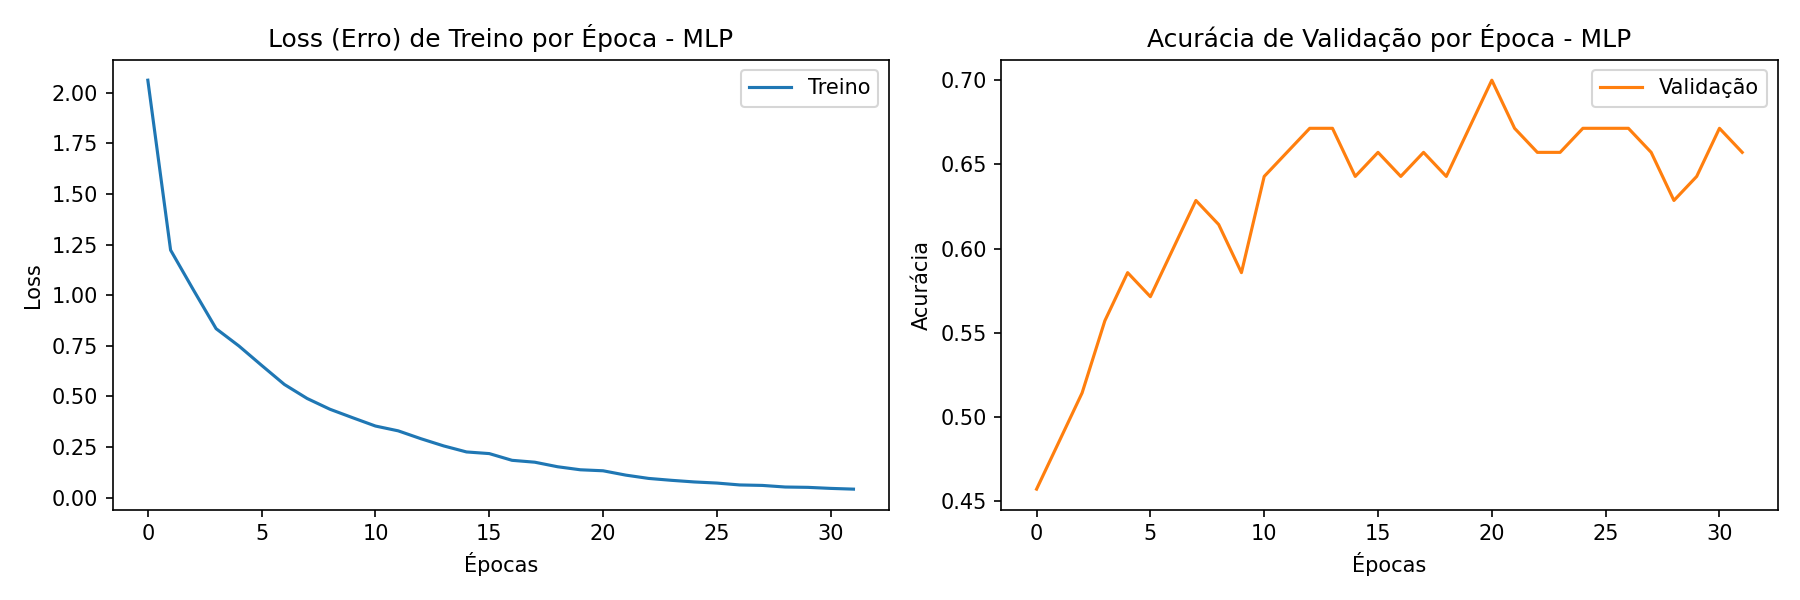
\includegraphics[width=\columnwidth]{mlp_training_curves.png}
        \caption{Curvas de perda (treino) e acurácia (validação) por época para o modelo tabular MLP.}
        \label{fig:mlp_curves}
    \end{figure}

    \begin{figure}[h]
        \centering
        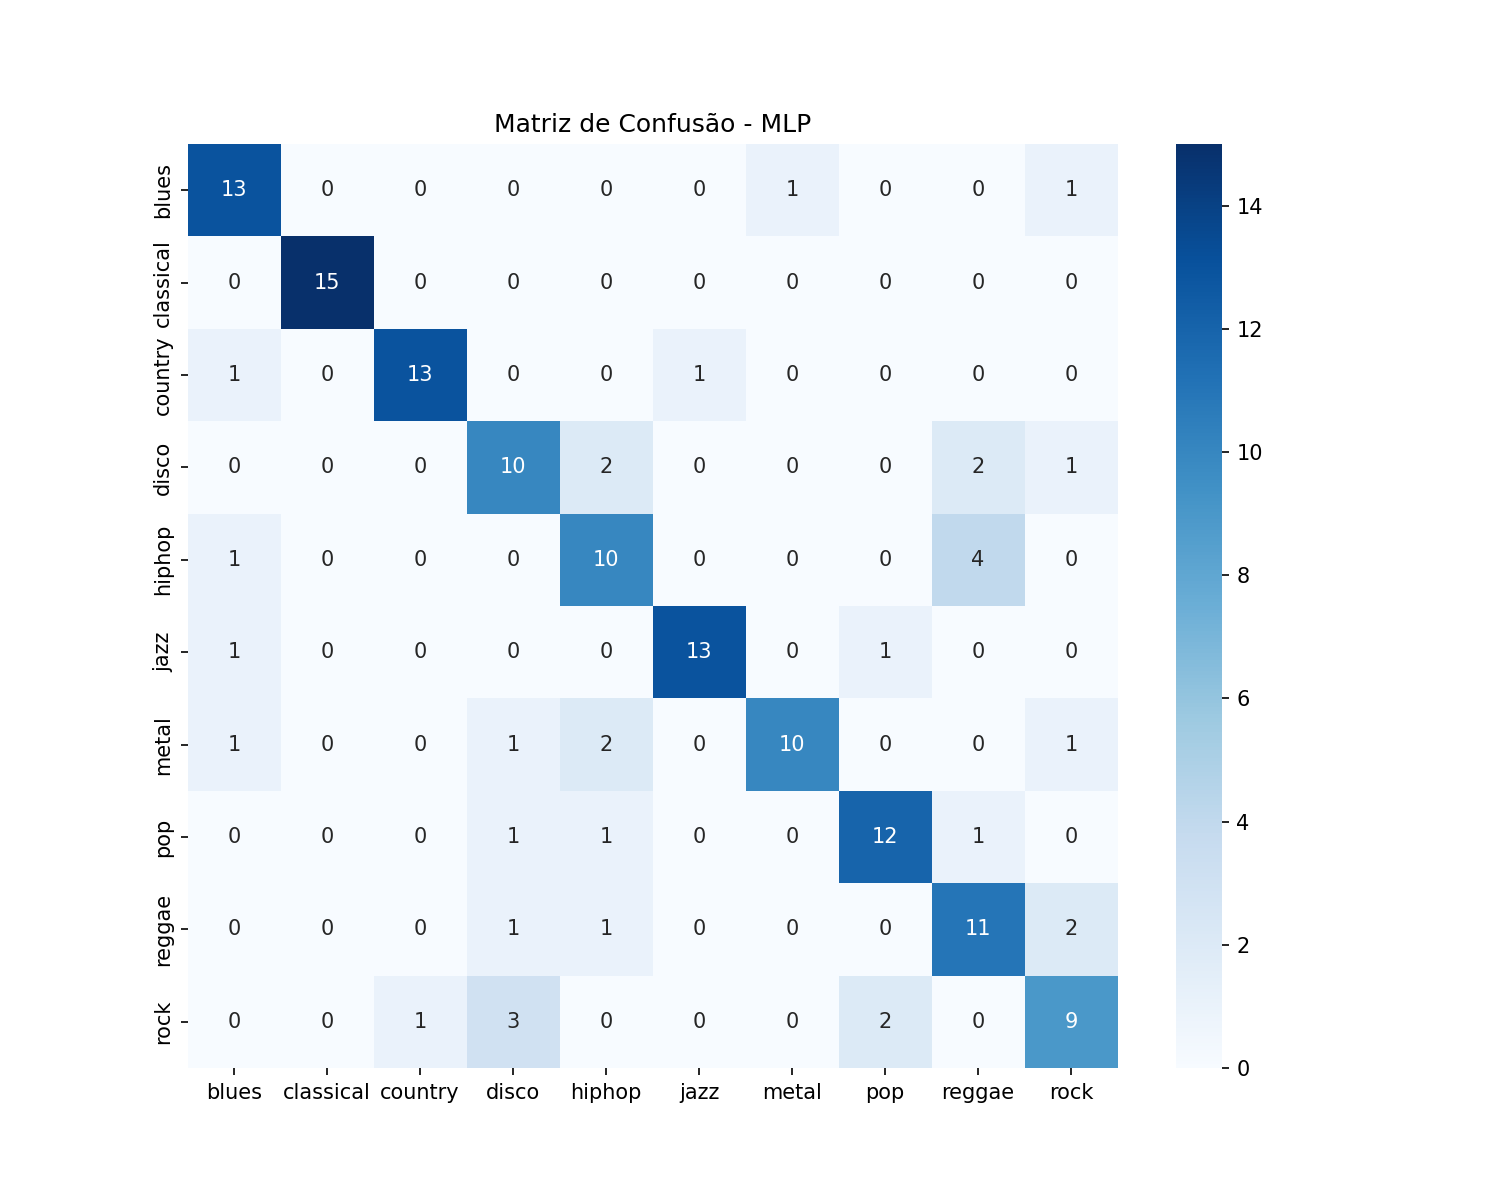
\includegraphics[width=0.9\columnwidth]{confusion_matrix_mlp.png}
        \caption{Matriz de confusão do MLP no conjunto de validação.}
        \label{fig:mlp_cm}
    \end{figure}

    \begin{figure}[h]
        \centering
        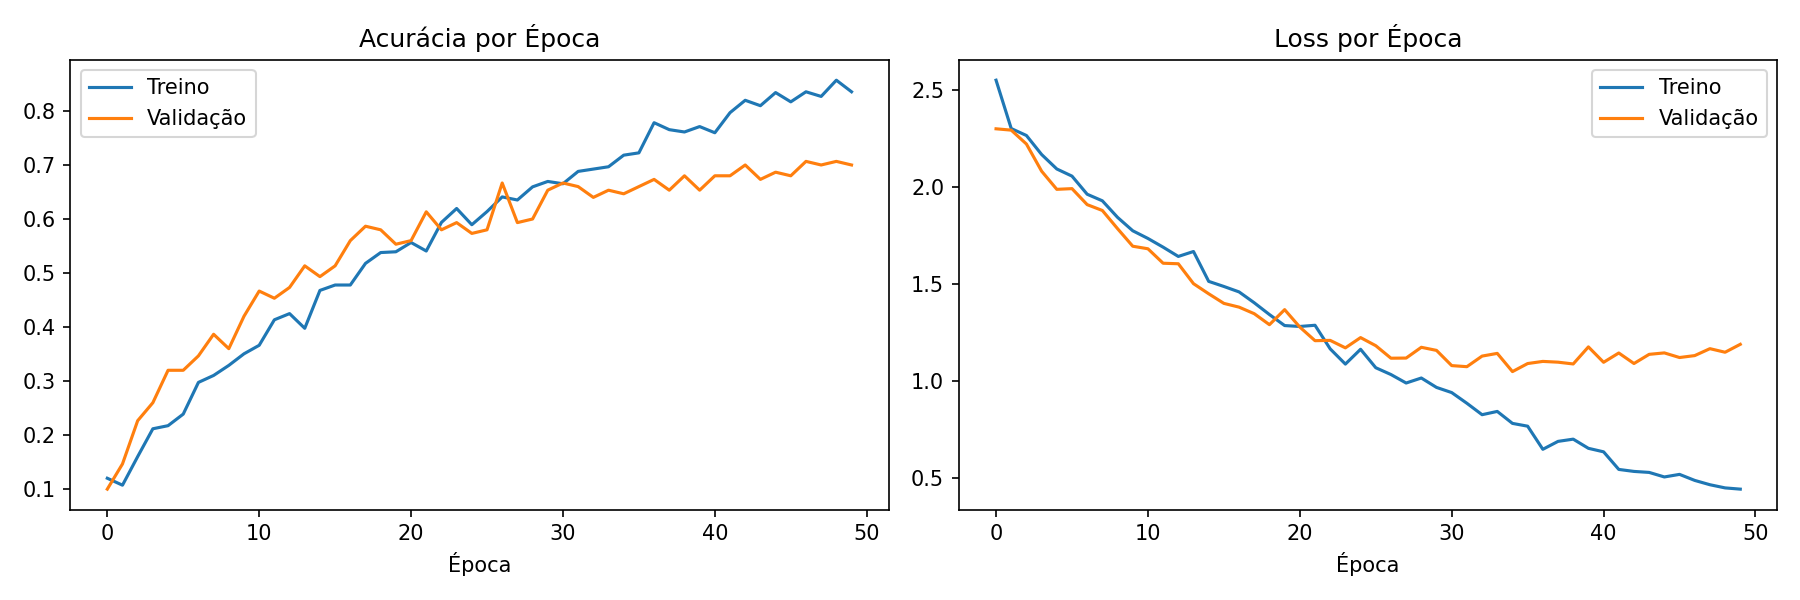
\includegraphics[width=\columnwidth]{cnn_training_curves.png}
        \caption{Curvas de acurácia e perda por época da CNN (treino e validação).}
        \label{fig:cnn_curves}
    \end{figure}

    \begin{figure}[h]
        \centering
        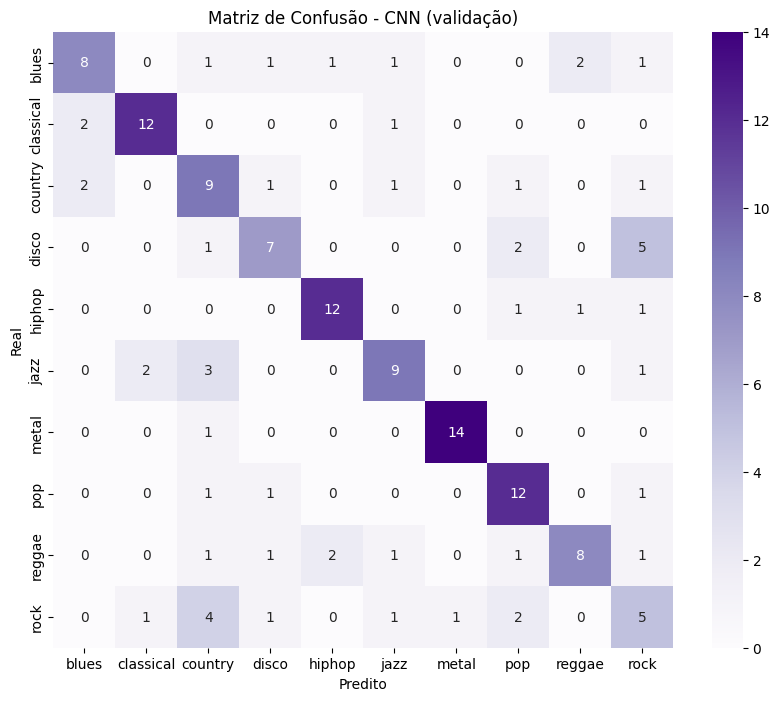
\includegraphics[width=0.9\columnwidth]{confusion_matrix_cnn.png}
        \caption{Matriz de confusão da CNN no conjunto de validação.}
        \label{fig:cnn_cm}
    \end{figure}
    
    
    % -------------------------------------------------------
    % VI. DISCUSSÃO
    % -------------------------------------------------------
    \section{Discussão}
    Os resultados indicam que o uso de descritores extraídos analiticamente (MFCCs) superou a extração autônoma de atributos espaciais da CNN para a tarefa proposta e as restrições impostas pelo dataset. Como os coeficientes de Mel refletem intimamente a percepção auditiva humana da forma do envelope espectral (timbre geral da faixa), a rede MLP obteve excelentes desempenhos para separar gêneros com instrumentações fundamentais muito dissimilares (como clássico vs metal).
    
    Por outro lado, a abordagem CNN sofreu uma restrição crítica: a quantidade de dados. Com apenas cerca de 700 espectrogramas para a fase de treinamento, a rede visual tendeu a se acomodar em \textit{overfitting} precocemente, possuindo informações insuficientes para derivar generalizações universais complexas que descritores de base matemática (como o MFCC) já entregam mastigados para a rede. Ainda assim, é possível notar, por meio das matrizes de erro, que descritores exclusivamente espectrais do MLP podem confundir compassos baseados fortemente em \textit{beats} sobrepostos (como a dificuldade entre \textit{hiphop} e \textit{reggae}), uma área temporal onde arquiteturas convolucionais alimentadas massivamente com dados poderiam se sobressair em trabalhos vindouros.
    
    % -------------------------------------------------------
    % VII. CONCLUSÃO
    % -------------------------------------------------------
    \section{Conclusão}
    Este trabalho comparou duas abordagens para classificação de gênero musical...
    
    % -------------------------------------------------------
    % REFERÊNCIAS
    % -------------------------------------------------------
    \begin{thebibliography}{99}
        
        \bibitem{tzanetakis2002}
        TZANETAKIS, G.; COOK, P. Musical genre classification of audio signals.
        \textit{IEEE Transactions on Speech and Audio Processing}, v. 10, n. 5, p. 293--302, 2002.
        
        \bibitem{logan2000}
        LOGAN, B. Mel Frequency Cepstral Coefficients for Music Modeling. In: \textit{International Symposium on Music Information Retrieval (ISMIR)}, 2000.
        
        \bibitem{costa2017}
        COSTA, Y. M. G.; OLIVEIRA, L. S.; SILLA JR., C. N. An evaluation of convolutional neural networks for music classification using spectrograms. \textit{Applied Soft Computing}, v. 52, p. 28--38, 2017.

        \bibitem{ioffe2015}
        IOFFE, S.; SZEGEDY, C. Batch normalization: Accelerating deep network training by reducing internal covariate shift. In: \textit{International Conference on Machine Learning (ICML)}, 2015. p. 448--456.
        
    \end{thebibliography}
    
\end{document}